\section*{CHAPTER 2: SYSTEM ANALYSIS AND DESIGN}
\addcontentsline{toc}{section}{\numberline{}CHAPTER 2: SYSTEM ANALYSIS AND DESIGN}
\setcounter{section}{2}
\setcounter{subsection}{0}
\setcounter{figure}{0}
\setcounter{table}{0}

This chapter translates the conceptual goals of the FootField platform into concrete engineering specifications. It details the functional requirements, identifies system actors, presents use case scenarios, and outlines the architectural and database designs. Additionally, it provides an in-depth review of the underlying technologies and architectural paradigms that form the foundation of the FootField platform.

\subsection{Software as a Service (SaaS) and Multi-Tenant Architecture}
Software as a Service (SaaS) is a cloud computing model where software applications are hosted by a third-party provider and made available to customers over the internet. Unlike the traditional on-premises software model, SaaS eliminates the need for organizations to install and run applications on their own computers or data centers, thereby reducing hardware acquisition, provisioning, and maintenance costs \cite{saas_architecture}.

A fundamental characteristic of a highly scalable SaaS application is its \textbf{Multi-Tenant Architecture}. In a multi-tenant environment, a single instance of the software and its underlying database serves multiple distinct customer organizations (tenants). There are several approaches to implementing multi-tenancy at the database level:
\begin{itemize}
    \item \textbf{Separate Databases:} Each tenant is allocated a completely isolated database. This provides the highest level of data security but incurs immense infrastructure costs and makes schema updates extremely difficult to manage across thousands of databases.
    \item \textbf{Shared Database, Separate Schemas:} All tenants share the same database instance, but each has its own schema (a distinct set of tables). This offers a middle ground between isolation and resource sharing.
    \item \textbf{Shared Database, Shared Schema:} All tenants share the exact same database and the same tables. Data isolation is achieved logically at the application level by associating every row of data with a unique identifier, commonly referred to as a \texttt{tenant\_id}. 
\end{itemize}

The FootField platform adopts the \textbf{Shared Database, Shared Schema} approach. This method was selected for its exceptional cost-efficiency and ease of maintenance. Every query executed by the backend must be strictly scoped using the \texttt{tenant\_id} to guarantee that tenants cannot access or modify each other's data.

\subsection{Backend Technologies: Node.js and Express.js}
Node.js is an asynchronous, event-driven JavaScript runtime built on Chrome's V8 JavaScript engine \cite{nodejs}. Traditional web servers, such as Apache, handle concurrent requests by spawning a new thread for each connection, which consumes significant memory. In contrast, Node.js operates on a single-threaded event loop. When it encounters an I/O operation (such as querying a database), it delegates the task to the operating system and continues processing other requests. Once the I/O operation completes, a callback function is placed in the event queue to be executed. This non-blocking architecture makes Node.js highly scalable and exceptionally well-suited for data-intensive, real-time applications like booking systems.

Express.js is a minimal and flexible web application framework running on top of Node.js \cite{expressjs}. It provides a robust set of features for routing HTTP requests, handling middleware, and serving static files. In this project, Express.js acts as the backbone of the Monolithic Hybrid architecture, managing RESTful API endpoints while concurrently serving the frontend HTML, CSS, and client-side JavaScript assets.

\subsection{Relational Databases and Query Builders}
For structured financial and operational data, relational database management systems (RDBMS) are the industry standard. MySQL, an open-source RDBMS, was chosen for its reliability, ACID (Atomicity, Consistency, Isolation, Durability) compliance, and widespread community support \cite{mysql}.

To interact with MySQL securely and efficiently from within the Node.js environment, the project utilizes Knex.js \cite{knexjs}. Knex.js is a "batteries-included" SQL query builder. Unlike Object-Relational Mappers (ORMs) which can sometimes obscure the underlying SQL and lead to performance bottlenecks, a query builder allows developers to write SQL-like syntax in JavaScript. Crucially, Knex.js automatically parametrizes queries, which is the primary defense mechanism against SQL Injection vulnerabilities. It also provides a robust migration system, allowing developers to version-control changes to the database schema.

\subsection{Artificial Intelligence and Function Calling Mechanics}
The integration of Artificial Intelligence transforms the platform from a passive tool into an active assistant. The platform leverages Google Gemini 1.5 Flash, an advanced Large Language Model (LLM) \cite{gemini_api}. 

While traditional chatbots rely on rigid, pre-programmed decision trees (e.g., "Press 1 for Booking, Press 2 for Support"), LLMs utilize Natural Language Processing (NLP) to understand the semantic intent behind a user's unstructured input. However, an LLM on its own is a "closed system"; it can generate text but cannot interact with external databases.

To overcome this, the project utilizes a relatively new paradigm known as \textbf{Function Calling} (or Tool Use). The workflow is as follows:
\begin{enumerate}
    \begin{sloppypar}
    \item \textbf{Definition:} The backend developer defines a set of functions (e.g., \texttt{check\_availability}, \texttt{create\_booking}) and provides the LLM with a JSON schema describing what these functions do and what parameters they require.
    \end{sloppypar}
    \item \textbf{Inference:} The user sends a message (e.g., "Book a 7-a-side field for tomorrow at 18:00"). The LLM analyzes the text, recognizes that the user wants to book a field, and instead of replying with text, it outputs a structured JSON object requesting the backend to execute the \texttt{create\_booking} function with the extracted parameters.
    \item \textbf{Execution:} The Node.js backend intercepts this request, executes the corresponding SQL query via Knex.js, and obtains the result (e.g., success or failure).
    \item \textbf{Resolution:} The backend sends the result back to the LLM. The LLM then synthesizes a natural language response (e.g., "I have successfully booked the 7-a-side field for you!") and presents it to the user.
\end{enumerate}
This mechanism bridges the gap between conversational AI and deterministic software execution.

\subsection{Cross-Platform Mobile Development with Capacitor}
Ionic Capacitor solves this problem by providing a cross-platform native runtime \cite{capacitor}. It allows developers to build mobile applications using standard web technologies (HTML, CSS, JavaScript). Capacitor acts as a bridge; it wraps the web application in a native WebView and exposes a set of JavaScript APIs that can communicate with native device hardware. In the context of the FootField platform, Capacitor is used to grant the web-based Tenant Admin dashboard access to the device's native camera, enabling the implementation of a high-speed QR code scanner for customer check-ins without the need for native code development.

\subsection{Cloud Storage and Persistent Media Management}
Deploying applications on Platform-as-a-Service (PaaS) providers like Render often involves working with ephemeral file systems. To achieve data persistence, the platform integrates with Cloudinary, a cloud-based media management service. By using the Cloudinary SDK, the backend automatically uploads files to the cloud and stores only the permanent URL in the MySQL database, ensuring that media assets remain accessible indefinitely.

\subsection{Real-time Alerts via Firebase Cloud Messaging (FCM)}
To ensure facility staff are immediately notified of new bookings, the platform utilizes Firebase Cloud Messaging (FCM). The backend utilizes the Firebase Admin SDK to trigger push notifications based on specific system events (e.g., successful payment). These notifications are delivered to the mobile application via a persistent connection, providing the "real-time" responsiveness required for a commercial service.

\subsection{Native Printing and Hardware Bridging}
The platform leverages the \texttt{cordova-plugin-printer} within the Capacitor environment to establish a bridge between the web interface and the mobile operating system's printing services. This allows the Tenant Admin dashboard to trigger native print dialogs and communicate with Bluetooth or Wi-Fi thermal printers directly from the mobile application.

The platform is designed to serve three distinct primary actors, each with specific privileges and functional needs. To better understand these requirements, we define the following user personas:

\subsubsection{User Persona: The Modern Facility Owner}
\textbf{Name:} Mr. Binh \\
\textbf{Goal:} Wants to reduce the time spent answering phone calls and managing a paper diary. He values real-time revenue visibility and a professional digital presence for his field business. \\
\textbf{Pain Point:} Double-bookings and "no-shows" that cause financial loss.

\subsubsection{User Persona: The Tech-Savvy Athlete}
\textbf{Name:} Tung \\
\textbf{Goal:} Wants to book a match quickly via his smartphone without talking to anyone. Prefers digital payments and needs instant confirmation. \\
\textbf{Pain Point:} Having to call multiple fields just to find an empty slot at 7 PM.

\subsubsection{User Persona: The Field Staff}
\textbf{Name:} Hoa \\
\textbf{Goal:} Needs a fast way to verify who has paid and who hasn't. Needs to check-in players quickly as they arrive. \\
\textbf{Pain Point:} Argumentative customers who claim they paid when the system shows they haven't.

\subsection{Requirements Analysis}
The platform is designed to serve three distinct primary actors, each with specific privileges and functional needs:

\textbf{1. Provider Admin (Super Admin):}
\begin{itemize}
    \item \textbf{Tenant Management:} Ability to create, suspend, or delete tenant (facility owner) accounts.
    \item \textbf{Package Management:} Ability to define subscription plans (e.g., Basic, Premium) that limit the number of fields or staff accounts a tenant can create.
    \item \textbf{Global Dashboard:} View aggregated revenue metrics and system-wide usage statistics.
\end{itemize}

\textbf{2. Tenant Admin (Facility Owner \& Staff):}
\begin{itemize}
    \item \textbf{Field Management:} Create and manage football fields, defining their type (5-a-side, 7-a-side) and hourly pricing strategies.
    \item \textbf{Schedule Viewer:} Access an interactive time-grid schedule to visually monitor all bookings across different fields on any given day.
    \item \textbf{QR Check-in:} Use the native mobile application to scan customer QR tickets and automatically update the booking status to "Completed".
    \item \textbf{Financial Reporting:} Generate daily and monthly revenue reports and print invoices.
\end{itemize}

\textbf{3. Customer (End-User):}
\begin{itemize}
    \item \textbf{Availability Search:} Browse available time slots for specific football fields.
    \item \textbf{AI Interaction:} Chat with the Gemini AI virtual assistant to request field recommendations or make bookings using natural language.
    \item \textbf{Online Payment:} Securely pay for bookings via VNPay.
    \item \textbf{Ticket Retrieval:} Receive and display an electronic QR code ticket upon successful booking.
\end{itemize}

\subsubsection{Non-Functional Requirements}
\begin{itemize}
    \item \textbf{Data Security:} Strict isolation of tenant data using the \texttt{tenant\_id} foreign key in all relevant database queries.
    \item \textbf{Performance:} API response times must remain under 500ms for standard database queries.
    \item \textbf{Availability:} The system must maintain 99.9\% uptime, facilitated by cloud-native deployment on Render and Aiven.
\end{itemize}

\begin{table}[htbp]
\centering
\begin{tabularx}{\textwidth}{|l|l|l|X|}
\hline
\rowcolor{LightCyan}
\textbf{Plan Tier} & \textbf{Monthly Price} & \textbf{Field Limit} & \textbf{Key Features} \\ \hline
Basic & 299,000 VND & Max 3 Fields & Dashboard, Field Mgmt, Basic Reports \\ \hline
Standard & 599,000 VND & Max 8 Fields & QR Check-in, Invoice Printing, Canteen Mgmt \\ \hline
Premium & 999,000 VND & Unlimited & AI Assistant, Camera Integration, Advanced CRM \\ \hline
\end{tabularx}
\caption{FootField SaaS Platform: Subscription Tiers and Features}
\label{tab:saas_tiers}
\end{table}

\begin{table}[htbp]
\centering
\begin{tabularx}{\textwidth}{|X|c|c|c|}
\hline
\rowcolor{LightCyan}
\textbf{Functional Capability} & \textbf{Provider} & \textbf{Tenant} & \textbf{Customer} \\ \hline
Manage Tenants \& Packages & [x] & [ ] & [ ] \\ \hline
Configure Fields \& Pricing & [ ] & [x] & [ ] \\ \hline
Conversational AI Booking & [ ] & [x] & [x] \\ \hline
Process VNPay Payments & [ ] & [ ] & [x] \\ \hline
Native QR Check-in & [ ] & [x] & [ ] \\ \hline
View Revenue Analytics & [x] & [x] & [ ] \\ \hline
\end{tabularx}
\caption{Actor-Role Permission Matrix}
\label{tab:permissions}
\end{table}

\subsection{Use Case Scenarios}

To visualize the interactions between the actors and the system, a comprehensive Use Case Diagram is established.

\begin{figure}[htbp]
    \centering
    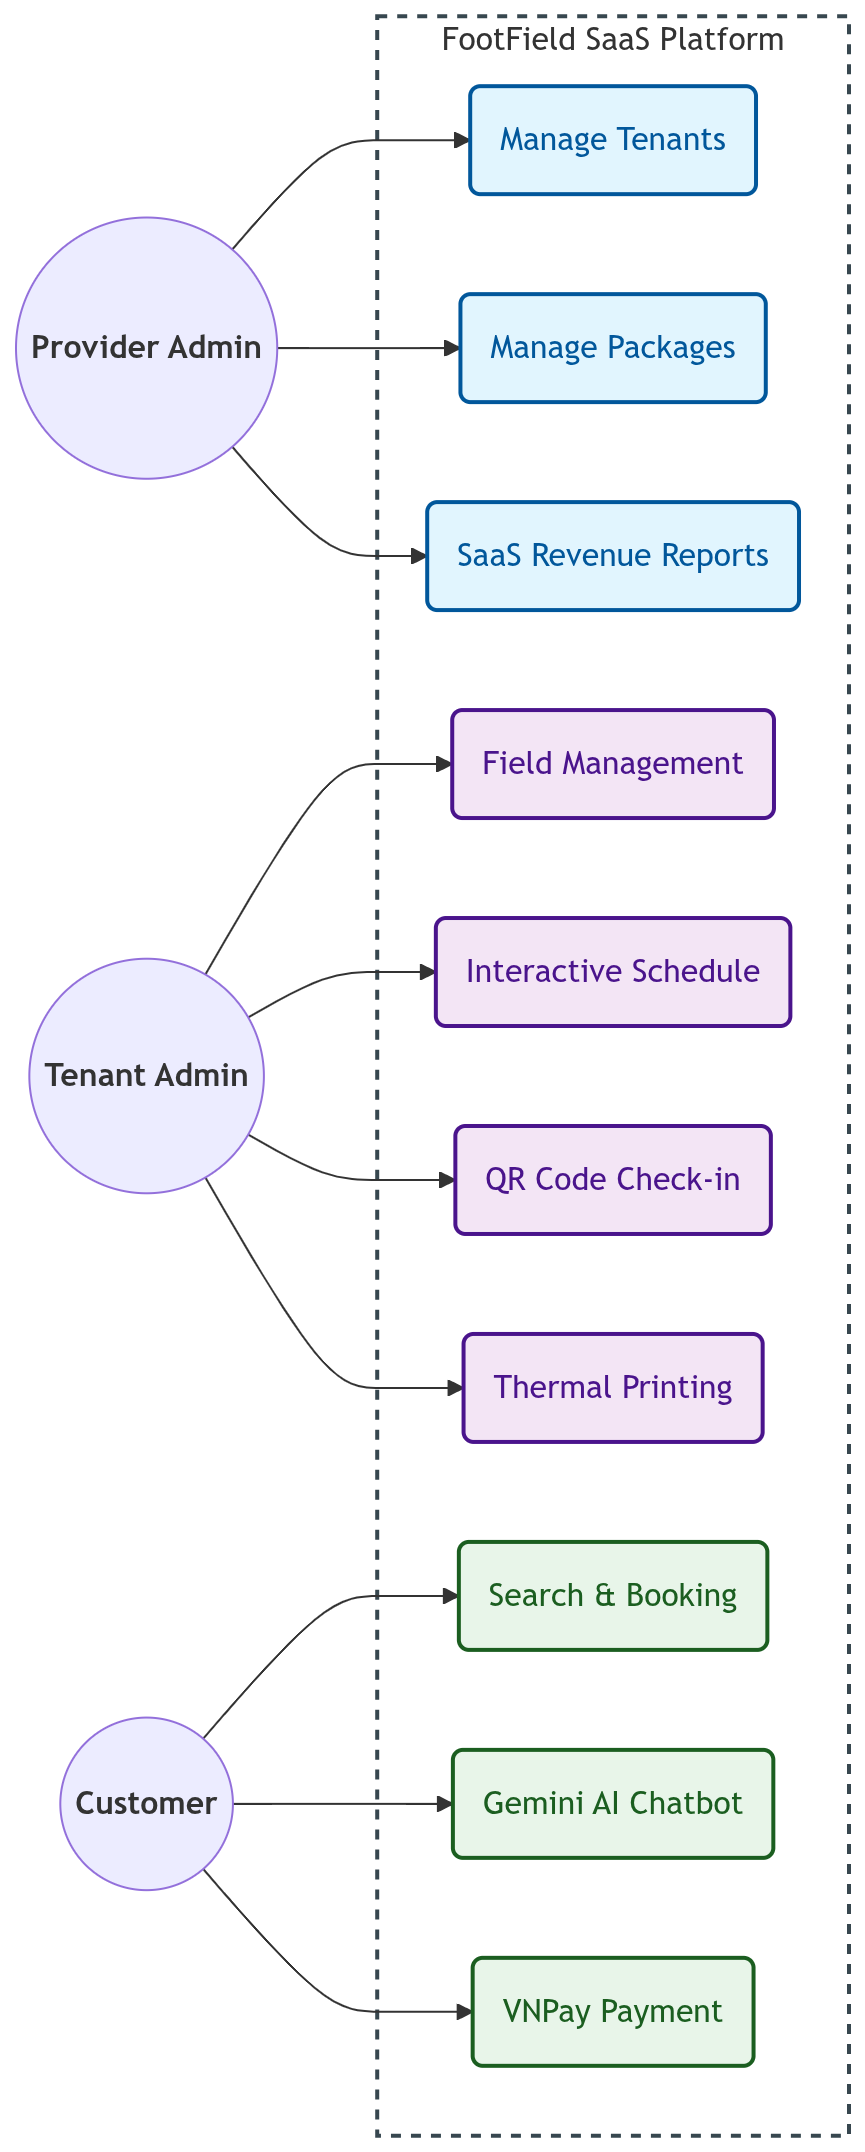
\includegraphics[width=0.58\textwidth]{Figures/usecase_diagram.png}
    \caption[General Use Case Diagram]{General Use Case Diagram for FootField SaaS Ecosystem}
    \label{fig:usecase}
\end{figure}

\subsubsection{Actor Definitions}
To understand the system boundaries, we must first define the roles and responsibilities of each actor interacting with the FootField platform:

\begin{itemize}
    \item \textbf{Provider Admin:} The highest authority in the ecosystem. Responsible for maintaining the infrastructure, managing the lifecycle of tenant accounts, and defining the commercial packages that govern system resource limits.
    \item \textbf{Tenant Admin (Field Owner):} The primary customer of the SaaS platform. This actor manages their own football facility, configures field availability, sets pricing strategies, and monitors staff performance and financial health.
    \item \textbf{Tenant Staff:} Subordinate accounts under a Tenant. They have limited access, focused on daily operations such as manual booking entry, customer check-in via QR codes, and processing on-site payments.
    \item \textbf{Customer:} The end-user who utilizes the public storefront or AI chatbot to browse field availability, execute bookings, and receive electronic tickets.
\end{itemize}

\subsubsection{Extended Functional Requirements}
Beyond the core features, the system implements several supporting functionalities to ensure a complete business workflow:

\begin{table}[htbp]
\centering
\begin{tabularx}{\textwidth}{|l|l|X|c|}
\hline
\rowcolor{LightCyan}
\textbf{ID} & \textbf{Requirement Name} & \textbf{Description} & \textbf{Priority} \\ \hline
FR-01 & Multi-tenant Login & Secure authentication for different actor types. & High \\ \hline
FR-02 & Dynamic Pricing & Ability to set different rates based on peak hours. & Medium \\ \hline
FR-03 & AI Conversational UI & Natural language processing for booking requests. & High \\ \hline
FR-04 & Automated Invoicing & Generate PDF/HTML receipts after successful payment. & Medium \\ \hline
FR-05 & Push Notifications & Real-time alerts for staff on new bookings. & Medium \\ \hline
FR-06 & QR Code Generation & Unique encrypted identifiers for each booking. & High \\ \hline
FR-07 & Revenue Analytics & Visual charts for daily/monthly financial tracking. & High \\ \hline
\end{tabularx}
\caption{Detailed Functional Requirements and Prioritization}
\label{tab:detailed_reqs}
\end{table}

\subsubsection{Detailed Use Case: AI-Assisted Booking}
\begin{itemize}
    \item \textbf{Goal:} To allow customers to book a field using natural language without navigating complex UI grids.
    \item \textbf{Primary Actor:} Customer.
    \item \textbf{Precondition:} The customer has accessed the specific tenant's storefront and has a stable internet connection to reach the Google Gemini API.
    \item \textbf{Main Success Scenario:}
    \begin{enumerate}
        \item Customer initiates a conversation: "Check if the 5-a-side field is free tonight at 8 PM."
        \item The system extracts entities: \texttt{field\_type: 5-a-side}, \texttt{time: 20:00}, \texttt{date: today}.
        \item The AI calls the \texttt{check\_availability} internal tool.
        \item The database returns "Available".
        \item The AI responds: "Yes, it is available! Would you like me to book it for you? The price is 300,000 VND."
        \item Customer confirms: "Yes, please book it under my name, Luong, 0987654321."
        \item The AI calls the \texttt{create\_booking} tool.
        \item The system creates a record in "Pending" status and generates a VNPay payment link.
        \item The AI provides the link: "Done! Here is your payment link: [URL]. Your booking will be confirmed once paid."
    \end{enumerate}
    \item \textbf{Alternative Flow (Conflict):} If the slot is taken, the AI suggests the nearest available time or a different field size (7-a-side).
\end{itemize}

\subsubsection{Use Case: Management of Sport Facilities}
\begin{itemize}
    \item \textbf{Goal:} To allow Tenant Admins to dynamically add, edit, or remove football fields from their catalog.
    \item \textbf{Primary Actor:} Tenant Admin.
    \item \textbf{Main Success Scenario:}
    \begin{enumerate}
        \item Admin navigates to the "Fields" management tab.
        \item System displays a list of currently active fields with their status (Available, Maintenance).
        \item Admin clicks "Add New Field".
        \item Admin enters details: Field Name (e.g., "Sân 3"), Type (5v5), Base Price (250k VND/h).
        \item Admin uploads an image of the field (handled via Cloudinary).
        \item System validates the data and persists it to the database, ensuring the \texttt{tenant\_id} is correctly associated.
        \item The new field becomes immediately available for booking on the customer storefront.
    \end{enumerate}
\end{itemize}

\subsubsection{Use Case: Financial Reporting and Analytics}
\begin{itemize}
    \item \textbf{Goal:} To provide Tenant Admins with data-driven insights into their business performance.
    \item \textbf{Primary Actor:} Tenant Admin.
    \item \textbf{Main Success Scenario:}
    \begin{enumerate}
        \item Admin opens the "Revenue" dashboard.
        \item System fetches data from the \texttt{bookings} table, filtering by \texttt{tenant\_id} and a date range.
        \item System calculates Total Revenue, Number of Bookings, and Most Popular Hours.
        \item Data is visualized using interactive charts (implemented via Chart.js on the frontend).
        \item Admin can export the report to a CSV or PDF format for physical accounting.
    \end{enumerate}
\end{itemize}

\subsection{Detailed UI/UX Design Principles}
The FootField platform adheres to modern web design standards, focusing on a "Mobile-First" and "Content-First" philosophy. The user interface is designed to be intuitive, requiring minimal training for facility staff.

\subsubsection{Color Palette and Typography}
A harmonious color scheme was selected to evoke a sense of professional sports and reliability:
\begin{itemize}
    \item \textbf{Success Green (\#16a34a):} Used for primary actions, confirmed bookings, and available slots.
    \item \textbf{Slate Gray (\#0f172a):} Used for high-contrast typography and deep backgrounds.
    \item \textbf{Vibrant Blue (\#3b82f6):} Used for info badges and navigation links.
\end{itemize}
Typography is handled by the "Barlow" font family, chosen for its condensed nature and excellent readability on small mobile screens.

\subsubsection{Interface Layouts}
\begin{enumerate}
    \item \textbf{The Slot Grid:} Instead of a simple list, bookings are displayed on a 2D time-grid. Each column represents a field, and rows represent hourly slots. This spatial representation allows managers to see "empty spaces" at a glance.
    \item \textbf{Floating Action Buttons (FAB):} In the mobile app, frequent actions like "Scan QR" are placed in a prominent floating button for easy thumb-access.
    \item \textbf{Skeleton Loading:} To improve perceived performance, the system uses skeleton loaders while fetching data from the Render-hosted API.
\end{enumerate}


\begin{table}[htbp]
\centering
\begin{tabularx}{\textwidth}{|l|l|X|}
\hline
\rowcolor{LightCyan}
\textbf{Tool Name} & \textbf{Parameters} & \textbf{System Action} \\ \hline
\texttt{check\_availability} & date, time & Queries the database for unoccupied slots on a specific date. \\ \hline
\texttt{create\_booking} & name, phone, date, time, field\_id & Inserts a new booking record and triggers the VNPay link generation. \\ \hline
\texttt{get\_pricing} & field\_id & Retrieves hourly rates and available promotions for a specific field. \\ \hline
\end{tabularx}
\caption{AI Service: Tool-Calling Schema Definitions}
\label{tab:ai_tools}
\end{table}

\subsubsection{Detailed Use Case: QR Code Check-in}
\begin{itemize}
    \item \textbf{Actor:} Tenant Staff
    \item \textbf{Precondition:} Staff is logged into the Capacitor Android app; Customer has a valid QR ticket.
    \item \textbf{Main Flow:}
    \begin{enumerate}
        \item Staff taps the "Scan QR" button on the mobile app.
        \item The Capacitor camera plugin opens the native device camera.
        \item Staff scans the customer's QR code.
        \item The app decodes the booking ID and sends an API request to the backend.
        \item The system verifies the booking status. If valid, it updates the status to "Completed".
        \item The app displays a success message to the staff.
    \end{enumerate}
\end{itemize}

\subsection{Database Design and ERD}

The database is built on a robust relational model to ensure data integrity. The core of the multi-tenant architecture is the enforcement of the \texttt{tenant\_id} relationship.

\begin{figure}[htbp]
    \centering
    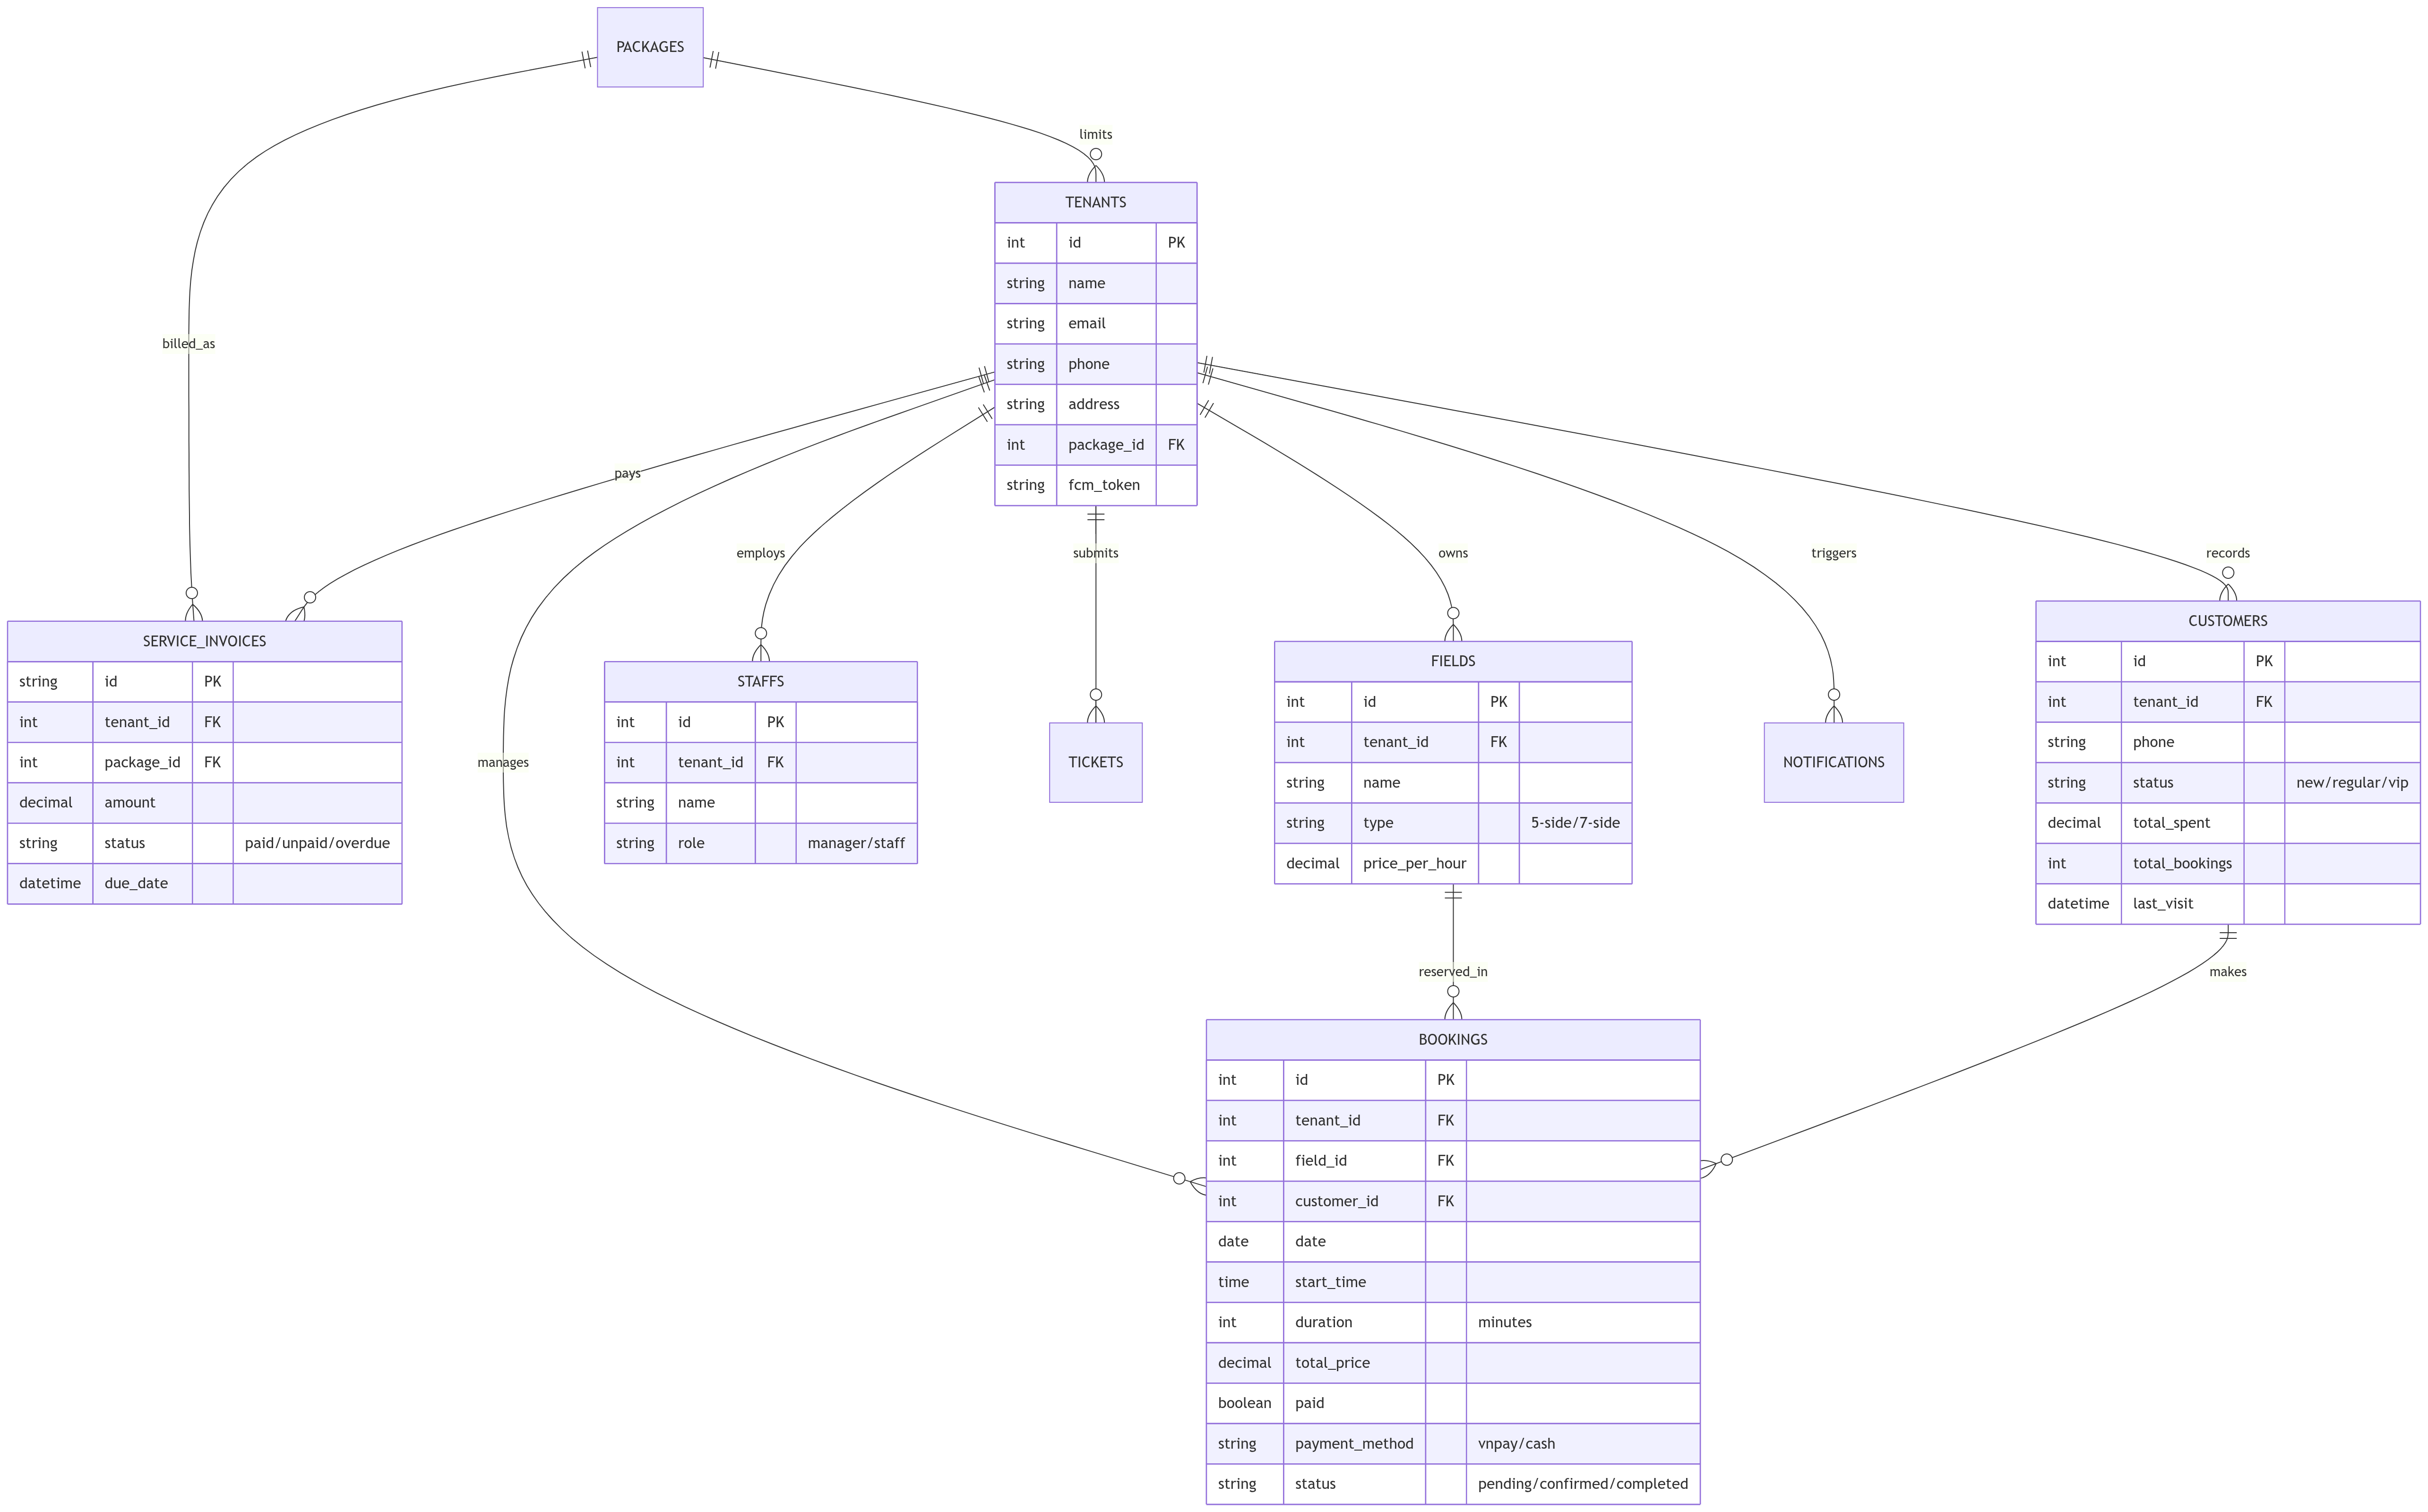
\includegraphics[width=1\textwidth]{Figures/erd_diagram.png}
    \caption[Entity-Relationship Diagram]{Optimized Entity-Relationship Diagram (ERD) with Multi-tenant isolation}
    \label{fig:erd}
\end{figure}

\subsubsection{Detailed Data Dictionary}
To ensure precise implementation, the database schema is strictly defined. Below are the specifications for the primary tables:

\textbf{1. Table: \texttt{tenants}}
\begin{table}[htbp]
\centering
\begin{tabularx}{\textwidth}{|l|l|l|X|}
\hline
\rowcolor{LightCyan}
\textbf{Column} & \textbf{Data Type} & \textbf{Constraint} & \textbf{Description} \\ \hline
id & VARCHAR(50) & Primary Key & Unique business identifier. \\ \hline
name & VARCHAR(100) & Not Null & Commercial name of the facility. \\ \hline
username & VARCHAR(50) & Unique & Login credential for the owner. \\ \hline
password & VARCHAR(255) & Not Null & Encrypted credentials. \\ \hline
package\_id & VARCHAR(20) & Foreign Key & Links to \texttt{packages.id}. \\ \hline
status & ENUM & 'active','suspended' & Account lifecycle state. \\ \hline
\end{tabularx}
\caption{Data Dictionary: Tenants Table}
\end{table}

\textbf{2. Table: \texttt{fields}}
\begin{table}[htbp]
\centering
\begin{tabularx}{\textwidth}{|l|l|l|X|}
\hline
\rowcolor{LightCyan}
\textbf{Column} & \textbf{Data Type} & \textbf{Constraint} & \textbf{Description} \\ \hline
id & INT & Primary Key & Auto-increment field ID. \\ \hline
tenant\_id & VARCHAR(50) & Foreign Key & Owner of the field. \\ \hline
name & VARCHAR(50) & Not Null & e.g., "Sân Số 1". \\ \hline
type & ENUM & '5v5','7v7' & Capacity classification. \\ \hline
price\_per\_hour & DECIMAL & Not Null & Base hourly rate. \\ \hline
status & VARCHAR(20) & Default: 'available' & 'available' or 'maintenance'. \\ \hline
\end{tabularx}
\caption{Data Dictionary: Fields Table}
\end{table}

\textbf{3. Table: \texttt{packages}}
\begin{table}[htbp]
\centering
\begin{tabularx}{\textwidth}{|l|l|l|X|}
\hline
\rowcolor{LightCyan}
\textbf{Column} & \textbf{Data Type} & \textbf{Constraint} & \textbf{Description} \\ \hline
id & VARCHAR(20) & Primary Key & Plan identifier (e.g., 'BASIC'). \\ \hline
name & VARCHAR(50) & Not Null & Display name of the plan. \\ \hline
max\_fields & INT & Not Null & Hard limit on number of fields. \\ \hline
price\_monthly & DECIMAL & Not Null & Subscription fee. \\ \hline
\end{tabularx}
\caption{Data Dictionary: Subscription Packages}
\end{table}

\textbf{4. Table: \texttt{payments}}
\begin{table}[htbp]
\centering
\begin{tabularx}{\textwidth}{|l|l|l|X|}
\hline
\rowcolor{LightCyan}
\textbf{Column} & \textbf{Data Type} & \textbf{Constraint} & \textbf{Description} \\ \hline
vnp\_txn\_ref & VARCHAR(100) & Primary Key & Unique transaction reference code (VNPay reference or BANK\_[id] for VietQR bank transfers). \\ \hline
booking\_id & INT & Foreign Key & Associated booking ID. \\ \hline
amount & DECIMAL & Not Null & Final paid amount. \\ \hline
bank\_code & VARCHAR(20) & Not Null & Issuing bank. \\ \hline
status & ENUM & 'success','fail' & Gateway response code. \\ \hline
\end{tabularx}
\caption{Data Dictionary: Financial Transactions}
\end{table}

\textbf{5. Table: \texttt{bookings}}
\begin{table}[htbp]
\centering
\begin{tabularx}{\textwidth}{|l|l|l|X|}
\hline
\rowcolor{LightCyan}
\textbf{Column} & \textbf{Data Type} & \textbf{Constraint} & \textbf{Description} \\ \hline
id & VARCHAR(50) & Primary Key & Unique booking reference. \\ \hline
tenant\_id & VARCHAR(50) & Foreign Key & Multi-tenant scope identifier. \\ \hline
field\_id & INT & Foreign Key & Associated football field. \\ \hline
date & DATE & Not Null & Targeted booking date. \\ \hline
start\_time & TIME & Not Null & Session start. \\ \hline
end\_time & TIME & Not Null & Session end. \\ \hline
status & ENUM & 'pending','confirmed','completed','cancelled' & Current state of the booking. \\ \hline
paid & BOOLEAN & Default: 0 & Payment verification flag. \\ \hline
qr\_code & VARCHAR(100) & Unique & Encrypted ticket string. \\ \hline
\end{tabularx}
\caption{Data Dictionary: Bookings Table}
\end{table}

\textbf{6. Table: \texttt{services}}
\begin{table}[htbp]
\centering
\begin{tabularx}{\textwidth}{|l|l|l|X|}
\hline
\rowcolor{LightCyan}
\textbf{Column} & \textbf{Data Type} & \textbf{Constraint} & \textbf{Description} \\ \hline
id & INT & Primary Key & Auto-increment ID. \\ \hline
tenant\_id & VARCHAR(50) & Not Null & Owner of the service. \\ \hline
name & VARCHAR(255) & Not Null & Name of item (e.g., Water, Ball). \\ \hline
price & INT & Not Null & Selling price. \\ \hline
category & VARCHAR(50) & Default: 'drink' & 'drink', 'food', 'rental'. \\ \hline
stock & INT & Default: 0 & Inventory quantity. \\ \hline
\end{tabularx}
\caption{Data Dictionary: Services (Canteen) Table}
\end{table}

\textbf{7. Table: \texttt{booking\_services}}
\begin{table}[htbp]
\centering
\begin{tabularx}{\textwidth}{|l|l|l|X|}
\hline
\rowcolor{LightCyan}
\textbf{Column} & \textbf{Data Type} & \textbf{Constraint} & \textbf{Description} \\ \hline
id & INT & Primary Key & Auto-increment ID. \\ \hline
booking\_id & VARCHAR(50) & Not Null & Associated booking. \\ \hline
service\_id & INT & Not Null & Associated service item. \\ \hline
quantity & INT & Not Null & Number of items purchased. \\ \hline
price\_at\_time & INT & Not Null & Price locked at time of sale. \\ \hline
\end{tabularx}
\caption{Data Dictionary: Booking Services (Orders) Table}
\end{table}

\subsection{System Activity and Workflows}
Beyond simple data models, the platform coordinates complex activities. Below is the detailed workflow for new tenant acquisition and customer booking.

\subsubsection{Workflow: Tenant Onboarding and Setup}
\begin{enumerate}
    \item \textbf{Registration:} The prospective owner fills a registration form on the Provider Portal.
    \item \textbf{Subdomain Allocation:} The system automatically provisions a unique subdomain (e.g., \texttt{vinhuni.footfield.app}).
    \item \textbf{Database Initialization:} The system injects a new \texttt{tenant\_id} into the shared tables.
    \item \textbf{Configuration:} The owner logs in and defines their field catalog, pricing rules, and operational hours.
    \item \textbf{Verification:} The platform owner verifies the business credentials and activates the account.
\end{enumerate}

\subsubsection{Workflow: Booking Cancellation and Refund}
To maintain fairness and reduce "no-shows," the system implements a strict cancellation policy:
\begin{itemize}
    \item \textbf{Grace Period:} Customers can cancel for a full refund up to 24 hours before the match.
    \item \textbf{Partial Refund:} Cancellations between 24 and 12 hours receive a 50\% credit back to their account.
    \item \textbf{No Refund:} Cancellations under 12 hours are non-refundable to compensate the field owner for the lost slot.
\end{itemize}
The refund process is handled via the VNPAY refund API, ensuring that money is returned to the original payment source automatically.

\subsection{System Sequence Diagrams}

Sequence diagrams illustrate the dynamic interaction between system components over time. These diagrams are crucial for understanding the asynchronous nature of the AI and Payment flows.

Sequence diagrams illustrate the dynamic interaction between system components over time. Two critical workflows are defined below.

\begin{figure}[htbp]
    \centering
    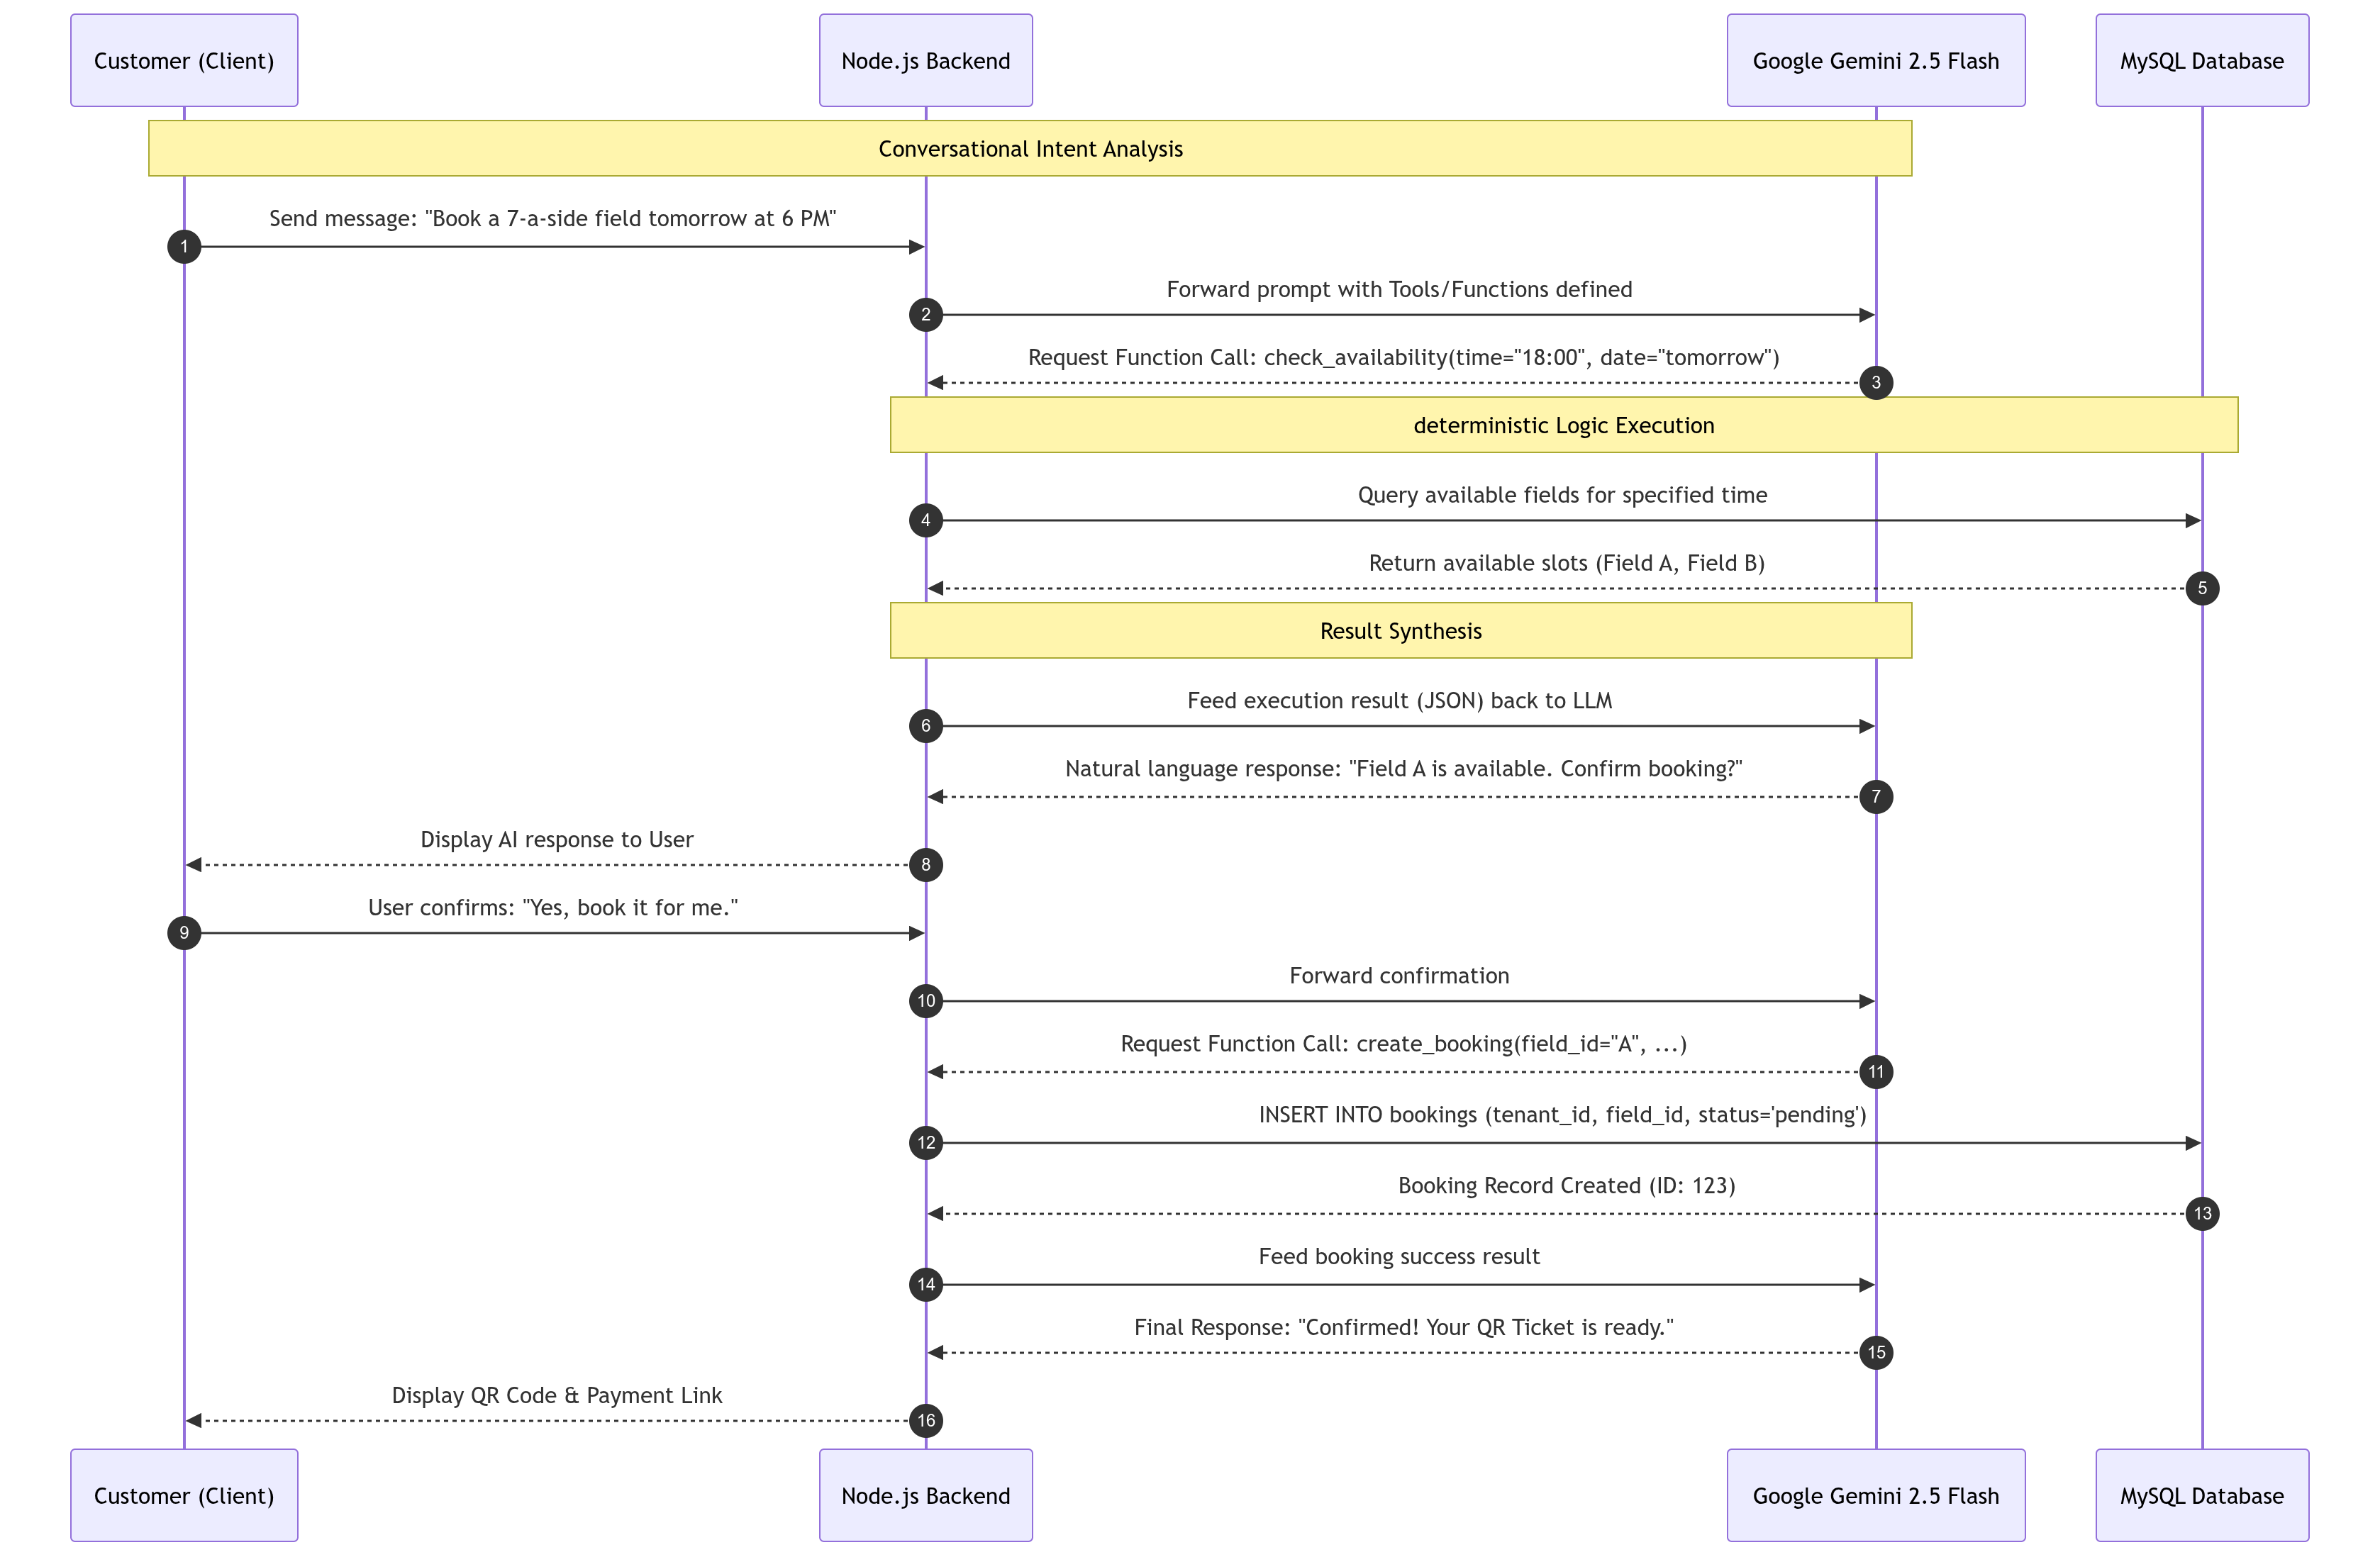
\includegraphics[width=1\textwidth]{Figures/seq_ai_booking.png}
    \caption[AI Booking Sequence]{Sequence Diagram: AI-Assisted Booking Workflow with LLM Function Calling}
    \label{fig:seq_ai}
\end{figure}